\documentclass{article}
\usepackage[numbers]{natbib}
\usepackage{amsmath}
\usepackage{graphicx}
\bibliographystyle{apsrev}

\newcommand{\lb}{\left(}
\newcommand{\rb}{\right)}
\newcommand{\db}[1]{{\lb {#1} \rb}}
\newcommand{\com}[2]{\left[ {#1},{#2} \right]}
\newcommand{\abs}[1]{\left| {#1} \right|}
\newcommand{\CC}{{\mathrm C}}
\newcommand{\dd}{{\ \mathrm d}}
\newcommand{\ee}{{\mathrm e}}
\newcommand{\ii}{{\mathbbm i}}
\newcommand{\OO}{{\mathrm O}}
\newcommand{\oo}{{\mathrm o}}
\newcommand{\ddfrac}[2]{\frac{{\mathrm d}{#1}}{{\mathrm d}{#2}}}
\newcommand{\pfrac}[2]{\frac{\partial{#1}}{\partial{#2}}}

\begin{document}
	\title{Social Force Models of Pedestrian Dynamics}
	\author{Boxiao Cao}
	\maketitle
	\section{Introduction}
        Everyone is pedestrian. Unfortunately, one pedestrian is killed every two hours and injured every eight minutes \cite{national2013traffic}.
        Pedestrian safety is a problem in transportation design.
        To have a better understanding of pedestrian behavior, mathematical models and computer simulations have been studied in past decades.
        Pedestrians could be simulated ether microscopically or macroscopically.
        
        In a microscopic model, each pedestrian is represented by one point, hence the movement of individual pedestrian is calculated.
        In a macroscopic model \cite{helbing1998fluid}, a point in simulation could represent a group of pedestrians.

        In this research, we focus on microscopic models.
        At time $t$, the pedestrian $i$ is at place $\vec{x}_i$, with velocity $\vec{v}_i$.
        Each pedestrians is looking for a convenient and comfortable way, minimizing travel time and avoiding obstacles, and make decision about his or her movement $\ddfrac{\vec{v}_i}{t}$.

        In order to calculate $\ddfrac{\vec{v}_i}{t}$, the social force model \cite{helbing1991mathematical,helbing1995social} was introduced.
        Based on idea from physics, in which acceleration is determined by force, the factors which determine pedestrian decision are called social force.
        Social forces are calculated independently, and the sum of all social forces determines the movement.

        The pedestrian $i$ wants to reach his or her destination $\vec{x}_i^0$.
        The desired direction is from current location to destination location
        $$
            \vec{e}_i = \frac{\vec{x}^0_i-\vec{x}_i}{\abs{\abs{\vec{x}^0_i-\vec{x}_i}}}
        $$
        There is a most comfortable speed $v_i^0$, and the desired velocity vector has magnitude of comfortable speed and direction of desired direction
        $$
            \vec{v}_i^0 = v_i^0\vec{e}_i^0
        $$
        The social force is proportional to the difference of desired velocity and current velocity, and is scaled by a relaxation time $\tau_i$
        $$
            \vec{f}_i =\frac{1}{\tau_i}\db{\vec{v}_i^0-\vec{v}_i}
        $$

        The pedestrian $i$ prefers to keep a distance to another pedestrian $j$,
        as there is a repulsion potential energy $V\db{r}$.
        The direction of repulsion force is awap from each other,
        $$
            \vec{e}_{ij} = \frac{\vec{x}_i-\vec{x}_j}{\abs{\abs{\vec{x}_i-\vec{x}_j}}}\
        $$
        $$
            \vec{f}_{ij} = \vec{e}_{ij}\pfrac{V}{r}\db{\abs{\abs{\vec{x}_i-\vec{x}_j}}}
        $$

        The potential function $V$ could not be measured directly, because pedestrian volunteers could not tell the quantity of potential or force he or she feels. Fortunately, the speed-density relation is measured from experiments. Starting from potential function $V$, one can mathematically solve the speed-density relation \cite{kretz2015inflection}. By comparing the speed-density relation measure and that solved, the potential function $V$ is albe to be calibrated.

        The $V\db{r}$, which is a function only about $r$, is called circular specification. This model works well under high-density conditions.

        When density is not high and movements are faster, a pedestrian $i$ begin to avoid standing in the way of another pedestrian $j$, in order to avoid a future collision. This implies that not only position but also velocity of $j$ has the effect of repulsion. The repulsion distance at moving direction is further than other direction, hence this is called elliptical specification I.  
        The elliptical specification II also consider the influence of velocity of $i$ \cite{johansson2007specification}.

        Human are not drawing ellipse when walking, instead, they predict whether the collision will happen or not (Figure \ref{img_collisionprediction}), slightly change the velocity, and evade the collision. Mathematically, the collision is able to be explicitly predicted \cite{zanlungo2011social} by positions and velocities. This method is like how human thinks. However, the collision prediction evasion involving three or more pedestrians are too complicated.

        \begin{figure}[htb]
            \centering
            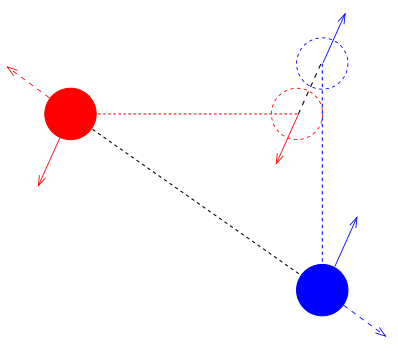
\includegraphics[natwidth=398,natheight=351,height=3cm]{img/collisionprediction.png}
            \caption{Collision prediction}
            \label{img_collisionprediction}
        \end{figure}

        The success of social force model is:
        decisions are made individually, while group behavior of large crowd is self-organized.
        Self-organized behaviors include shock waves, lane forming, circulating flow and clogging effects \cite{helbing2005self}.

    \section{Programming}
        In order to have the ability in monitoring and modifying social force model, I have writen my own code of social force.
        The source code is released under GPL license at https://github.com/antiphoton/pedestrian.

        The program contains a simulator and a viewer.
        The simulator is to generate pedestrian trajectories.
        The viewer is to display the trajectories.
        \subsection{Simulator}
            The simulator is writen in C++.
            \begin{itemize}
                \item{main.cpp} \\
                    This file is entry point of simulator.
                \item{mymath.cpp} \\
                    This file implements vector operations.
                    And also, this file contains compression algorithms, which helps making output file smaller.
                \item{mytime.cpp} \\
                    The time functions in C library is somewhat hard to use.
                    This file defines some friendly functions.
                \item{mympi.cpp} \\
                    The simulator is designed to run parallelly. This file controls the communication between CPUs.
                \item{reading.cpp} \\
                    The modules of simulator have a lot of parameters. Those parameter are not hard coded in source code, they are writen in input files. One can test different experiments by chaning input files, without needing to recompile simulator.
                \item{frame.cpp} \\
                    This file reads and manages the timestep of simulation.
                \item{gate.cpp} \\
                    The source gates are where pedestrians are created. The sink gates are where pedestrians evacuate to.
                    In this file, source gates decides when and where to create a new pedestrian, and sink gates decide if any pedestrian has already evacuated.
                \item{gravity.cpp} \\
                    This file calculates the shortest path from a pedestrian's current location to his or her destination. The current edge of shortest path determines the desied moving direction of a pedestrian.
                \item{person.cpp} \\
                    This file defines the pedestrian movement and interactions between pedestrians.
                \item{playground.cpp} \\
                    This file maintains the neighbour list.
                \item{wall.cpp} \\
                    This file calculates the interaction between a pedestrian and walls.
                \item{trajectory.cpp} \\
                    This file writes output of simulator. The output file is a JSON file.
            \end{itemize}
            The simulator reads parameters of experiment conditions, simulate pedestrian behaviors each time step, and print out the trajectoris of all pedestrians.
        \subsection{Viewer}
            Once the trajectory file is generated, it might be needed to be presented on different computers.
            In order to make a cross-platform viewer, the viewer is designed to run within a web browser.
            Hence the viewer is writen in Javascript.

            There is a draggable ruler to measure the distance.
            By playing with the trajectory forward, backward, faster, slower, frame by frame, one can have a convinient picture and intuitive feeling of the simulated pedestrian movement, and judge whether the simulated behaviors are like human behaviors.


    \section{Methods}
        With the framework of social force model and tool of simulation, it's time to add my own features into social force model.
        \subsection{Detour}
            Methods for repulsion have been studied in past researches, but collision avoidance is not the only action a pedestrian would take. A pedestrian needs not only keep distance from others, but also go to destination.
            When pedestrian $i$ is facing another pedestrian $j$ in front of $i$, the best choice of $i$ is not step backward, but bypass $j$.

            The desired moving direction of $i$ is $\vec{e}_i$, the direction from $j$ to $i$ is $\vec{e}_{ij}$, the detour is needed when $j$ is in front of $i$
            $$
                \vec{e}_i \cdot \vec{e}_{ij} < 0
            $$

            In order to bypass $j$, the force on $i$ should be perpendicular to $\vec{e}_{ij}$, in the direction of
            $$
                \frac{\vec{f}_i}{\abs{\abs{\vec{f}_i}}} = \vec{e}_{ij} \times \db{ \vec{e}_i \times \vec{e}_{ij} }
            $$
        \subsection{Full stop}
            The idea of social force model is from idea of molecular dynamics.
            One pedestrian is treated as one particle (molecule), following Newton's Law.
            However, there is a significant difference between the behaviors of pedestrians and those of particles.
            Particles oscillate at equilibrium position, however, pedestrians fully stop at equilibrium position.
            After entering full stop state, the pedestrian begin to look around, and stand at the same position until an accepted gap is observed.

            In reality, a pedestrian falls in the full stop state as long as his or her velocity is $\vec{0}$. In computer simulation, the velocity of a pedestrian is updated one time step by one time step, hence the velocity does not change continuously. The velocity is usually changed from $+0.01\rm{m/s}$ to $-0.01\rm{m/s}$ in one time step, skipping $0.00\rm{m/s}$.

            In an update procedure of a pedestrian, the velocity before update is $\vec{v}\db{t}$, and the velocity after update is $\vec{v}\db{t+\mathrm{d}t}$. A full stop is detected when $\vec{v}\db{t}$ and $\vec{v}\db{t+\mathrm{d}t}$ are not in the same direction
            $$
                \vec{v}\db{t} \cdot \vec{v}\db{t+\mathrm{d}t} \le 0
            $$

            In order to quantify gap acceptability, not only the force of current time step but also the forces of past a few seconds should be taken into consideration.
            When the forces of past few seconds are pointing to the same direction, the movement of that direction is regarded as continous prefered, thus the gap at that direction is accepted.
            The forces are pointing to the same direction if the magnitude of weight average vector of the forces is consideralby not equal to zero.
            To get a smoother result, the average is weighted by a decay function $g\db{\xi}$. In some words, the condition for an acceptable gap is
            $$
                \abs{\abs{ \int_0^\infty \vec{f}\db{t-\xi}g\db{\xi} \dd \xi} }\ge F_0 {\int_0^\infty g\db{\xi} \dd \xi}
            $$
            where $F_0$ is the pre-set starting force magnitude for a pedestrian.

            This method requires both storing and accessing the whole history of force, which is low efficiency at both space and time.
            Fortunately, carefully selected $g\db{\xi}$ could solve this problem. It is noted that
            \begin{equation*}
                \begin{aligned}
                    I\db{t+\Delta t}
                        &=
                            \int_0^\infty \vec{f}\db{t+\Delta t-\xi} \ee^{\xi/\tau} \dd \xi \\
                        &=
                            \int_0^{\Delta t} \vec{f}\db{t+\Delta t-\xi} \ee^{\xi/\tau} \dd \xi
                            +
                            \int_{\Delta t}^\infty \vec{f}\db{t+\Delta t-\xi} \ee^{\xi/\tau} \dd \xi \\
                        &=
                            \vec{f}\db{t+\Delta t} \Delta t
                            +
                            \int_{\Delta t}^\infty \vec{f}\db{t+\Delta t-\xi} \ee^{\xi/\tau} \dd \xi \\
                        &=
                            \vec{f}\db{t+\Delta t} \Delta t
                            +
                            \int_0^\infty \vec{f}\db{t-\xi} \ee^{\db{\xi-\Delta t}/\tau} \dd \xi \\
                        &=
                            \vec{f}\db{t+\Delta t} \Delta t
                            +
                            I\db{t} \ee^{-\Delta t/\tau} \\
                \end{aligned}
            \end{equation*}
            By selecting $g\db{\xi}=\ee^{\xi/\tau}$, integration $I\db{t+\Delta t}$ could be calculated efficiently.
        \section{Results}

            \begin{figure}[htb]
                \centering
                \begin{tabular}{cc}
                    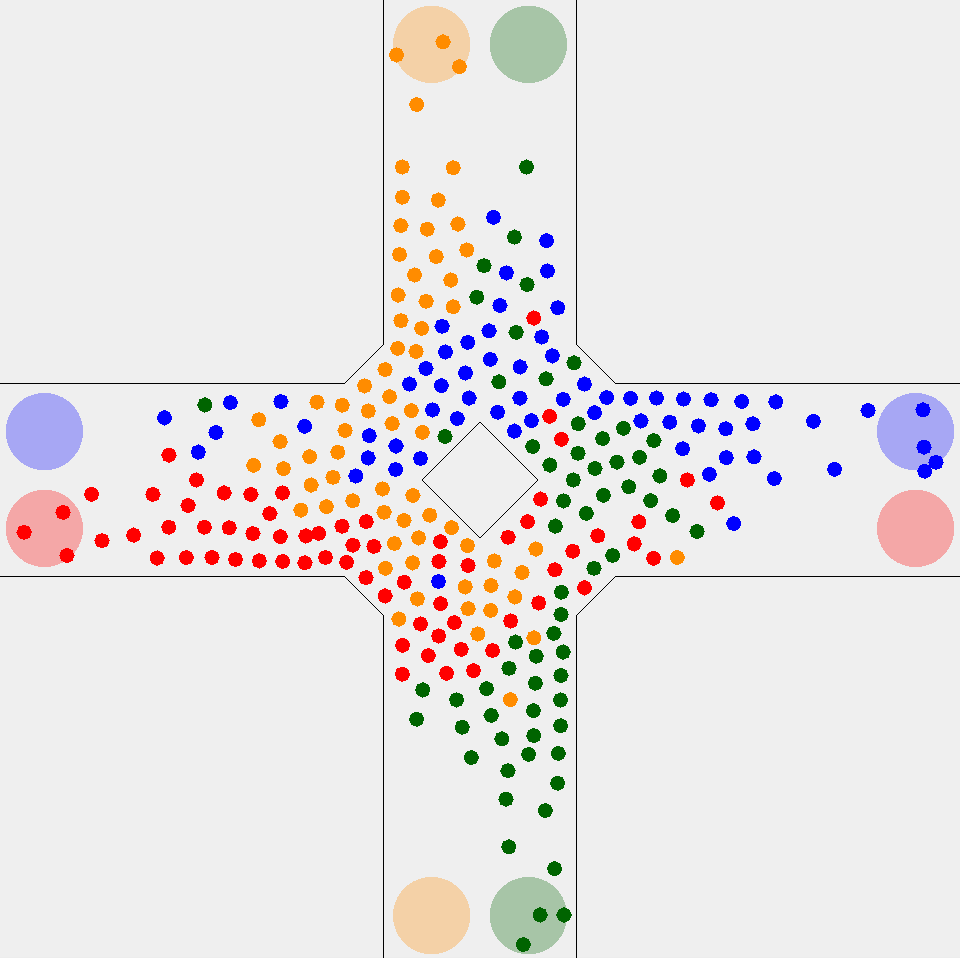
\includegraphics[natwidth=960,natheight=958,width=6cm]{img/cross1.png} &
                    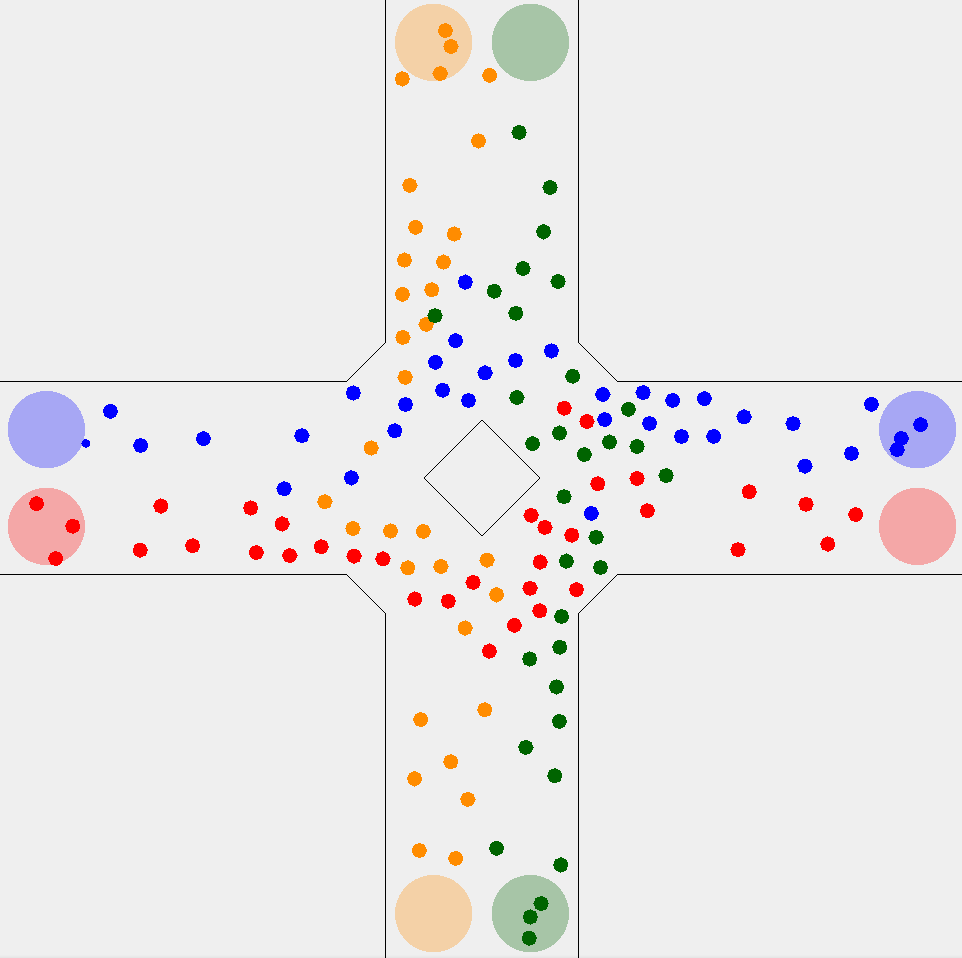
\includegraphics[natwidth=962,natheight=958,width=6cm]{img/cross2.png} \\
                    (a) Unmodified & (b) With detour and stop \\
                \end{tabular}
                \caption{Simulation of crossroad}
                \label{img_cross}
            \end{figure}

            Figure \ref{img_cross} shows the social force model simulation of crossroad flows. The size of playground was $25\rm{\ m}\times 25\rm{\ m}$.
            Red were moving from left to right. Green were moving from bottom to top.  Blue were moving from right to left.  Yellow were moving from top to bottom.
            The snapshot was taken after pedestrian moving for 60 seconds.
            In figure \ref{img_cross}(a), the majority part of pedestrians were blocked at the center, even though some pedestrians are trying to form circulating flow, they were not able to go through the crowd. In figure \ref{img_cross}(b), pedestrians were bypassing each other easily.

            \begin{figure}[htb]
                \centering
                \begin{tabular}{cc}
                    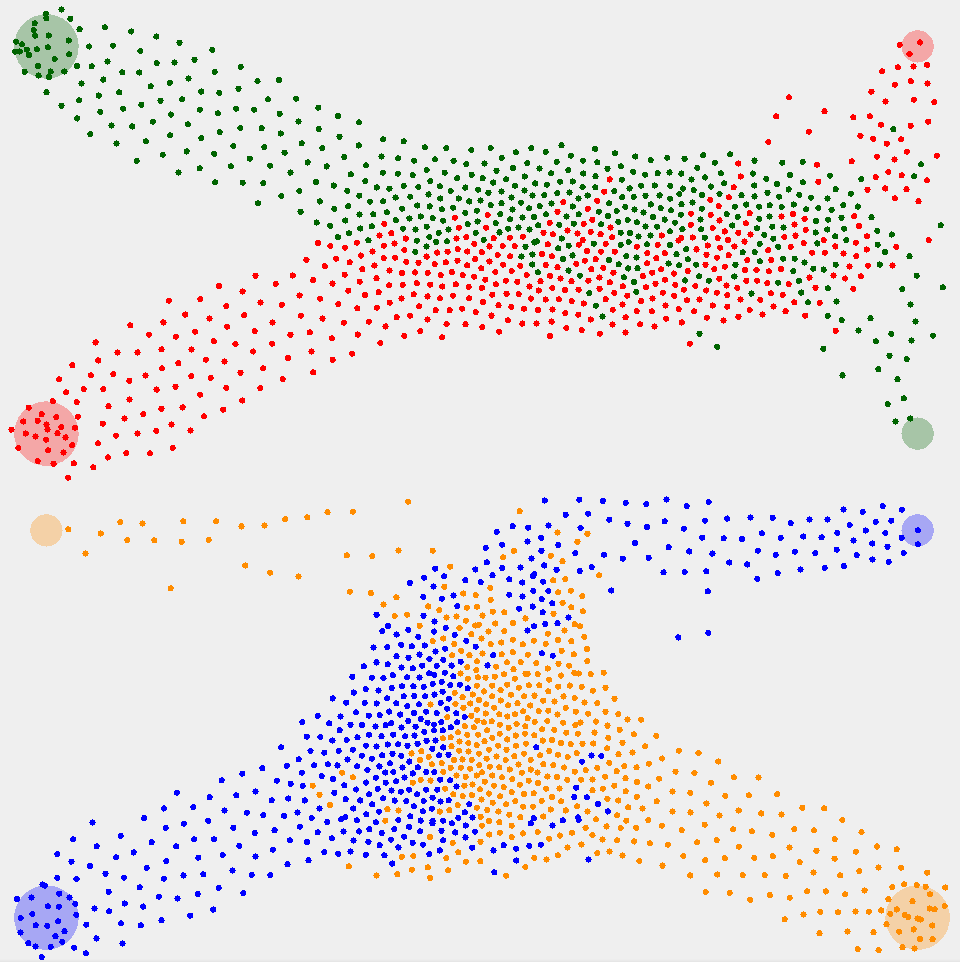
\includegraphics[natwidth=960,natheight=962,width=6cm]{img/stripe1.png} &
                    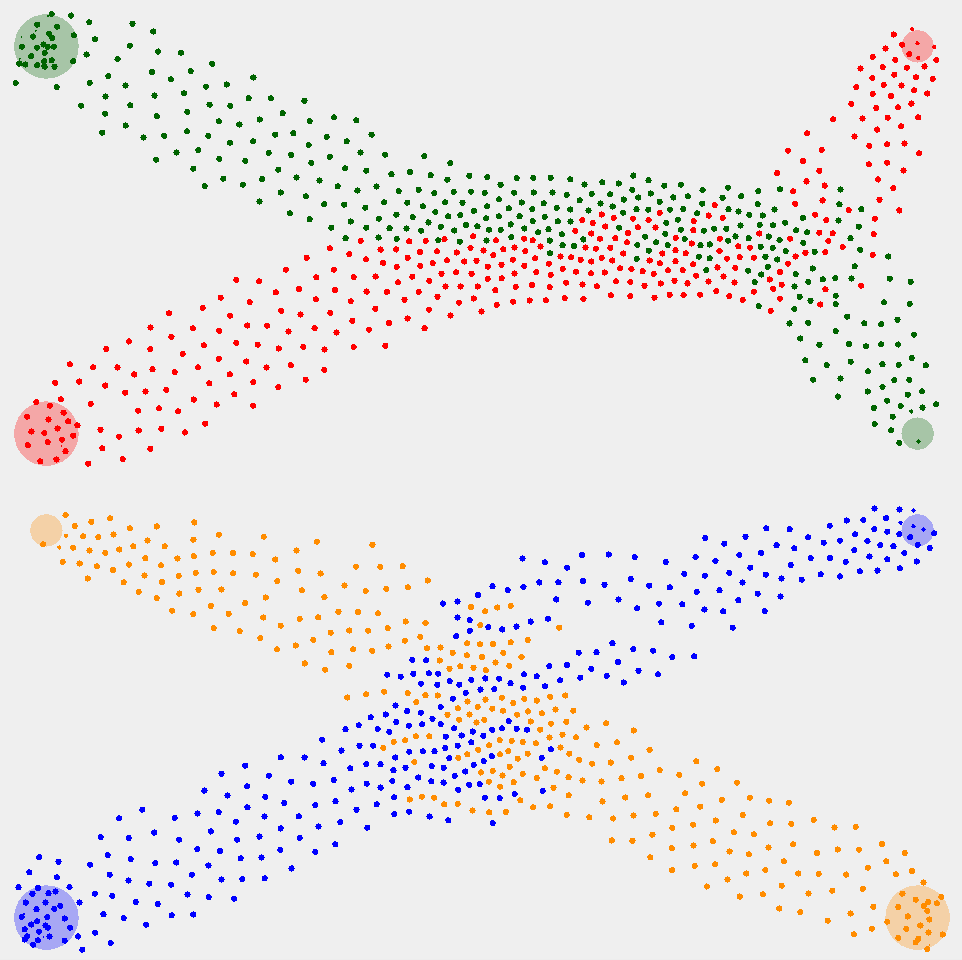
\includegraphics[natwidth=962,natheight=960,width=6cm]{img/stripe2.png} \\
                    (a) Unmodified & (b) With detour and stop \\
                \end{tabular}
                \caption{Simulation of intersecting streams}
                \label{img_stripe}
            \end{figure}

            Figure \ref{img_stripe} shows the social force model simulation of intersecting pedestrian streams. The size of playground was $60\rm{\ m}\times 60\rm{\ m}$.
            Red and green were moving from left to right. Blue and yellow were moving from bottom to top.
            The snapshot was taken after pedestrian moving for 100 seconds.
            In figure \ref{img_stripe}(a), the majority part of pedestrians were blocked at the center, even though some pedestrians are trying to form stripes, they were not able to go through the crowd. In figure \ref{img_stripe}(b), pedestrians were bypassing each other easily, and stripes were clearly formed.
        \section{Conclusion \& Discussion}
            Adding human features to social force model leads to better results of social force model. After calibration, it can help us get more accurate pedestrian behaviors and help us design more safety and efficiency pedestrian transportation facilities.
	\renewcommand\refname{Reference}
	\bibliography{main}
\end{document}

